%\subsection{Schema generale: associazione dei nodi al flusso dati con estensioni}
%\begin{figure}[H]
%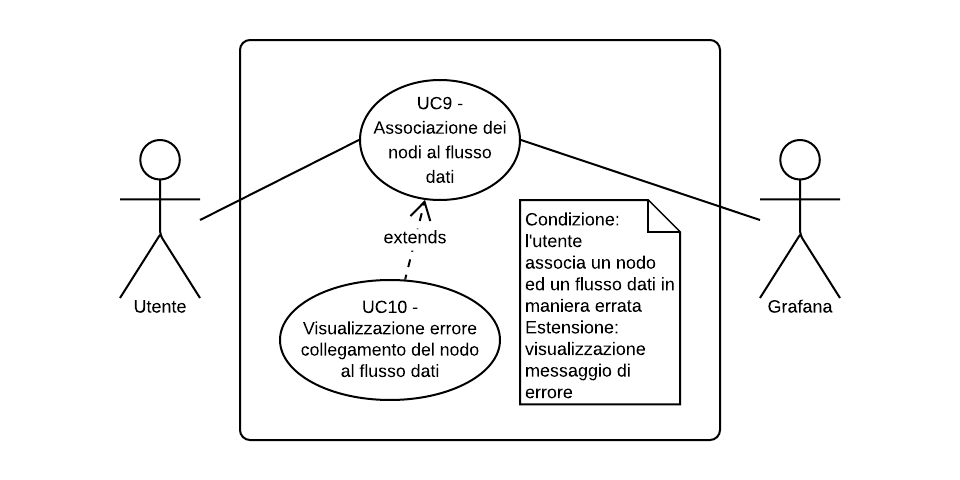
\includegraphics{img/UC9 - Schema generale.png}
%\caption{Schema generale: associazione dei nodi al flusso dati con estensioni}
%\end{figure}
\subsection{UC9 - Associazione dei nodi al flusso dati}
\begin{figure}[H]
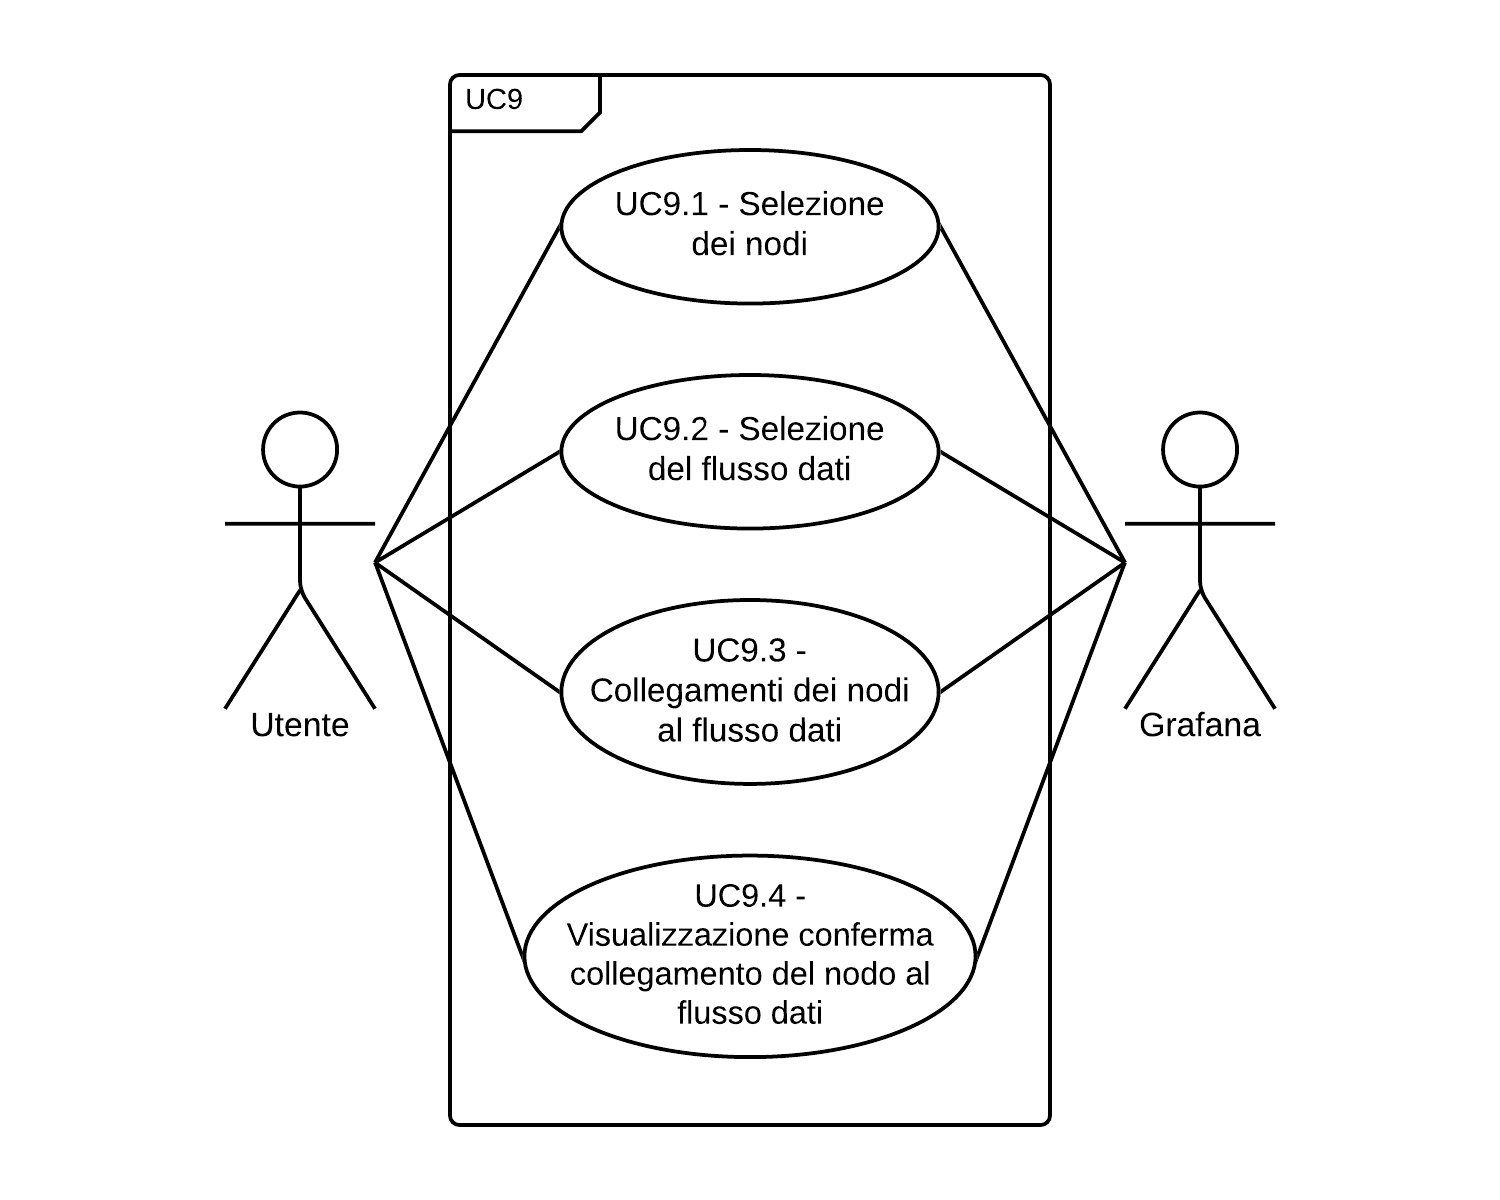
\includegraphics{img/UC9_-_Associazione_dei_nodi_al_flusso_dati.png}
\caption{Diagramma degli use case di UC9}
\end{figure}
\begin{itemize}
	\item \textbf{Codice identificativo}: UC9;
	\item \textbf{Titolo}: associazione dei nodi al flusso dati;
	\item \textbf{Attori primari}: utente;
	\item \textbf{Attori secondari}: Grafana\glo;
	\item \textbf{Descrizione}: l'utente esegue l'associazione dei nodi individuati per l'attività di previsione;
	\item \textbf{Precondizioni}: l'utente è autenticato nel sistema software Grafana\glosp, ha avviato il plug-in e ha caricato il file JSON con i dati di addestramento;
	\item \textbf{Postcondizioni}: i nodi sono stati associati al flusso dati con successo;
	\item \textbf{Scenario principale}: 
		\begin{itemize}
			\item selezione del nodo (UC9.1);
			\item selezione del flusso dati (UC9.2);
			\item collegamenti dei nodi al flusso dati (UC9.3);
			\item visualizzazione conferma collegamento del nodo al flusso dati (UC9.4).
		\end{itemize}
	\item \textbf{Estensioni}:
		\begin{itemize}
			\item se l'utente crea un abbinamento non valido tra un nodo ed il flusso dati viene visualizzato un messaggio di errore (UC10).
		\end{itemize}
\end{itemize}

\subsubsection{UC9.1 - Selezione dei nodi}
\begin{itemize}
	\item \textbf{Codice identificativo}: UC9.1;
	\item \textbf{Titolo}: selezioni del nodi;
	\item \textbf{Attori primari}: utente;
	\item \textbf{Attori secondari}: Grafana\glo;
	\item \textbf{Descrizione}: l'utente seleziona i nodi tramite il plug-in;
	\item \textbf{Precondizioni}: l'utente ha avviato correttamente il plug-in;
	\item \textbf{Postcondizioni}: l'utente ha selezionato correttamente il nodo;
	\item \textbf{Scenario principale}: l'utente seleziona il nodo da associare al flusso di dati.
\end{itemize}

\subsubsection{UC9.2 - Selezione del flusso dati}
\begin{itemize}
	\item \textbf{Codice identificativo}: UC9.2;
	\item \textbf{Titolo}: selezione del flusso dati;
	\item \textbf{Attori primari}: utente;
	\item \textbf{Attori secondari}: Grafana\glo;
	\item \textbf{Descrizione}: l'utente seleziona il flusso di dati tramite il plug-in;
	\item \textbf{Precondizioni}: l'utente ha avviato correttamente il plug-in;
	\item \textbf{Postcondizioni}: l'utente ha selezionato correttamente flusso dati;
	\item \textbf{Scenario principale}: l'utente seleziona il flusso dati a cui viene associato il nodo.
\end{itemize}

\subsubsection{UC9.3 - Collegamenti dei nodi al flusso dati}
\begin{itemize}
	\item \textbf{Codice identificativo}: UC9.3;
	\item \textbf{Titolo}: collegamenti dei nodi al flusso dati;
	\item \textbf{Attori primari}: utente;
	\item \textbf{Attori secondari}: Grafana\glo;
	\item \textbf{Descrizione}: l'utente esegue il collegamento dei nodi al flusso dati;
	\item \textbf{Precondizioni}: l'utente ha avviato correttamente il plug-in, ha selezionato i nodi ed il flusso dati;
	\item \textbf{Postcondizioni}: l'utente ha collegato correttamente i nodi al flusso dati;
	\item \textbf{Scenario principale}: l'utente seleziona il flusso dati a cui viene associato il nodo.
\end{itemize}

\subsubsection{UC9.4 - Visualizzazione conferma collegamento del nodo al flusso dati}
\begin{itemize}
	\item \textbf{Codice identificativo}: UC9.4;
	\item \textbf{Titolo}: visualizzazione conferma collegamento del nodo al flusso dati;
	\item \textbf{Attori primari}: utente;
	\item \textbf{Attori secondari}: Grafana\glo;
	\item \textbf{Descrizione}: l'utente visualizza la conferma di collegamento del nodo al flusso dati avvenuta con successo;
	\item \textbf{Precondizioni}: l'utente ha avviato il plug-in e ha eseguito il collegamento dei nodi al flusso dati;
	\item \textbf{Postcondizioni}: l'utente ha visualizzato la conferma del collegamento dei nodi al flusso dati;
	\item \textbf{Scenario principale}: l'utente visualizza la conferma del collegamento dei nodi al flusso dati.
\end{itemize}